\documentclass{article}


\usepackage{arxiv}
\usepackage{algorithm,algpseudocode}

\usepackage[utf8]{inputenc} % allow utf-8 input
\usepackage[T1]{fontenc}    % use 8-bit T1 fonts
\usepackage{hyperref}       % hyperlinks
\usepackage{url}            % simple URL typesetting
\usepackage{booktabs}       % professional-quality tables
\usepackage{amsfonts}       % blackboard math symbols
\usepackage{nicefrac}       % compact symbols for 1/2, etc.
\usepackage{microtype}      % microtypography
\usepackage{lipsum}
\usepackage{amsmath}
\usepackage{amssymb}
\usepackage{textcomp}
\usepackage[dvipsnames]{xcolor}
\usepackage{graphicx}
\usepackage{subcaption}
\usepackage{bbold}
\usepackage{bm}
\newcommand{\CO}{\mathcal{O}}
\usepackage{wrapfig}
\newcommand\subfig[2]{{Fig.~\ref{#1}{#2}}}
\newcommand\fig[1]{{Fig.~\ref{#1}}}
\usepackage[super]{nth}
\usepackage{dirtytalk}
\usepackage{braket}
%\usepackage{blindtext}
%\usepackage{tcolorbox}
%\usepackage{graphicx}

\usepackage{empheq}
\usepackage[most]{tcolorbox}
\tcbset{highlight math style={boxsep=1mm,colback=blue!30!red!10!white}}

\title{Préparation de Windows 10 pour le TP}


\author{
Pour toute question, veuillez contacter\\
 Juliane U. Klamser\\%\thanks{website}\\
  Gulliver,  ESPCI\\
  Paris \\
  \texttt{Juliane.Klamser@espci.psl.eu} \\
}

\begin{document}
\maketitle

\tableofcontents

%\begin{abstract}
%Bla bla
%\end{abstract}


% keywords can be removed
%\keywords{First keyword \and Second keyword \and More}
\section{Logiciels anti-virus}
Les logiciels anti-virus sont les plus susceptibles de bloquer la préparation de votre ordinateur. Il existe deux scénarios
\begin{enumerate}
\item Vous pouvez désinstaller votre logiciel anti-virus et le réinstaller ultérieurement, une fois que toutes les étapes de préparation sont terminées.
\item Vous ne pouvez pas désinstaller votre logiciel anti-virus.
\end{enumerate}

Comment procéder dans les différents scénarios ?
\begin{enumerate}
\item Dans le premier scénario, désinstallez votre anti-virus et redémarrez votre ordinateur. Après avoir redémarré votre ordinateur, assurez-vous que le logiciel anti-virus n'est plus là.
\item Dans le deuxième scénario:
\begin{enumerate}
\item Si le logiciel anti-virus est Kaspersky: Settings $\rightarrow$ Additional $\rightarrow$ Network $\rightarrow$ Monitored ports: Monitor selected ports only $\rightarrow$ Select $\rightarrow$ Disable the following two: HTTPS  and HTTP with Port 80. 
\begin{figure}[H]
\begin{subfigure}[c]{0.7\textwidth}
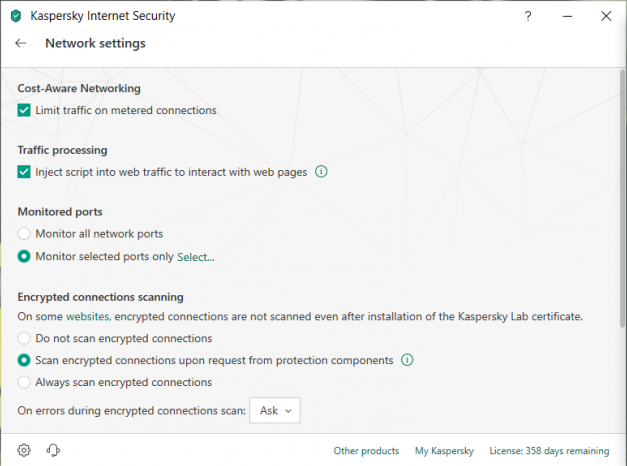
\includegraphics[width=1\textwidth]{Plots/Kasp1.png}
\subcaption{Settings $\rightarrow$ Additional $\rightarrow$ Network $\rightarrow$ Monitored ports: Monitor selected ports only}
\end{subfigure}
\begin{subfigure}[c]{0.3\textwidth}
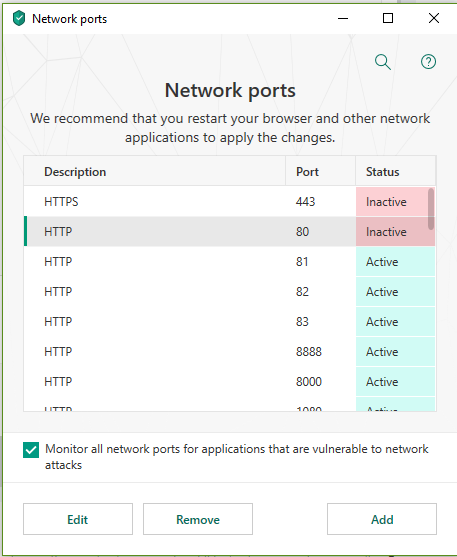
\includegraphics[width=1\textwidth]{Plots/Kasp2.png}
\subcaption{Disable the following two: HTTPS  and HTTP with Port 80}
\end{subfigure}
\caption{Preparation of Kaspersky settings.}
\end{figure}
\item S'il s'agit d'un autre programme anti-virus, nous devrons d'abord essayer sans modifier les paramètres. Si vous êtes bloqué au cours des étapes suivantes, contactez \href{mailto:example@example.com}{juliane.klamser@espci.psl.eu}
\end{enumerate}
\end{enumerate}
\section{Activer la fonction : Windows Subsystem for Linux}
Allez dans le menu Start et recherchez PowerShell. Exécutez-le en tant qu'administrateur :
\begin{figure}[H]
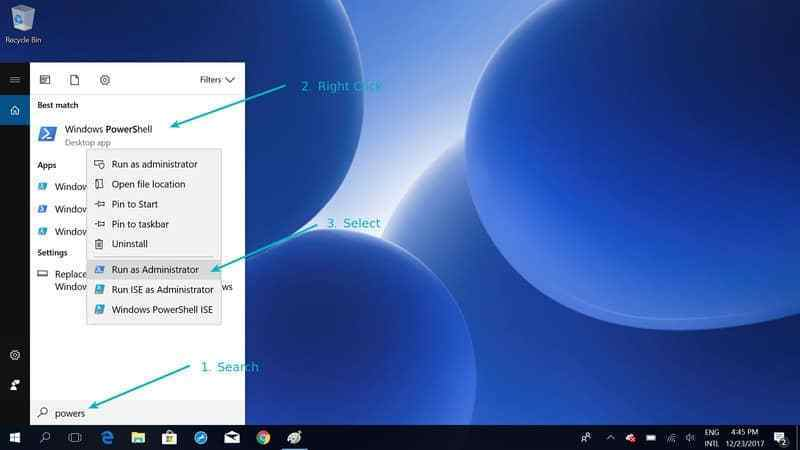
\includegraphics[width=1\textwidth]{Plots/Powershell-Ubuntu-install.jpg}
%\caption{Preparation of Kaspersky settings.}
\end{figure}
Après l'ouverture du PowerShell, copiez et passez la ligne suivante dans le terminal PowerShell et appuyez sur entrée:

\begin{tcolorbox}[width=\textwidth,colback={purple},title={PowerShell terminal},outer arc=0mm,colupper=white]    
    Enable-WindowsOptionalFeature -Online -FeatureName Microsoft-Windows-Subsystem-Linux
\end{tcolorbox}
Il vous sera demandé de confirmer votre choix. Tapez Y ou appuyez sur la touche Entrée :
\begin{figure}[H]
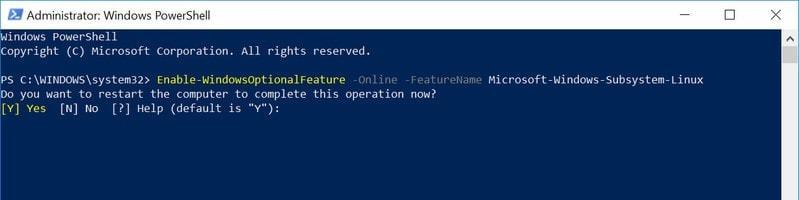
\includegraphics[width=1\textwidth]{Plots/Powershell-Ubuntu-install-2.jpg}
%\caption{Preparation of Kaspersky settings.}
\end{figure}

Maintenant, on devrait vous demander de redémarrer. Même si on ne vous le demande pas, vous devez redémarrer votre système.

\section{Installation de l'application Ubuntu}
Installez une application appelée Ubuntu à partir de l'App Store microsoft (suivez ce lien \href{https://www.microsoft.com/en-us/p/ubuntu/9nblggh4msv6?activetab=pivot:overviewtab}{https://www.microsoft.com/en-us/p/ubuntu/9nblggh4msv6?activetab=pivot:overviewtab}).

Cette application sera votre terminal. 

Ouvrez l'application pour terminer l'installation. 
Il vous sera demandé d'insérer un nom d'utilisateur et d'insérer un mot de passe. 

\textbf{Attention} : Lorsque vous entrez le mot de passe, vous ne verrez rien. Il semble que rien ne se passe. Une fois que vous avez tapé votre mot de passe, appuyez sur "Enter". Il vous sera demandé de confirmer votre mot de passe.

\textbf{Note} : Vous devez noter ce nom d'utilisateur et le mot de passe à un endroit où vous ne le perdez pas. Dans ce document, nous appellerons ce nom d'utilisateur et ce mot de passe Ubuntu-Username et Ubuntu-password.

\section{Installation des paquets nécessaires}

Tout ce qui suit doit être fait dans votre nouveau terminal ubuntu. Ouvrez l'application. Vous pouvez écrire dans ce terminal. Notez que vous ne pouvez vous déplacer entre les lettres qu'avec les touches fléchées de votre clavier. 

Copiez et collez les commandes suivantes (l'une après l'autre) dans le terminal ubuntu et confirmez avec ENTER. Chaque fois que vous confirmez l'une des commandes suivantes avec ENTER, une installation démarre.  Attendez que l'installation se termine avant de taper la commande suivante. Vérifiez attentivement s'il n'y a pas de messages d'erreur après une installation. En cas de messages d'erreur, contactez \href{mailto:example@example.com}{juliane.klamser@espci.psl.eu}.

\begin{enumerate}
\item commande:
\begin{tcolorbox}[width=\textwidth,colback={blue},title={ubuntu terminal},outer arc=0mm,colupper=white]    
    sudo apt-get update
\end{tcolorbox}
Vous devrez peut-être entrer votre Ubuntu-password. Vous devrez peut-être confirmer avec "Y". Attendez que l'installation soit terminée. 
\item commande:
\begin{tcolorbox}[width=\textwidth,colback={blue},title={ubuntu terminal},outer arc=0mm,colupper=white]    
    sudo apt install g++
\end{tcolorbox}
Vous devrez peut-être entrer votre Ubuntu-password. Vous devrez peut-être confirmer avec "Y". Attendez que l'installation soit terminée. 
\item commande:
\begin{tcolorbox}[width=\textwidth,colback={blue},title={ubuntu terminal},outer arc=0mm,colupper=white]    
    sudo apt-get install libcairo2-dev
\end{tcolorbox}
Vous devrez peut-être entrer votre Ubuntu-password. Vous devrez peut-être confirmer avec "Y". Attendez que l'installation soit terminée. 
\item commande:
\begin{tcolorbox}[width=\textwidth,colback={blue},title={ubuntu terminal},outer arc=0mm,colupper=white]    
    sudo apt-get install gnuplot
\end{tcolorbox}
Vous devrez peut-être entrer votre Ubuntu-password. Vous devrez peut-être confirmer avec "Y". Attendez que l'installation soit terminée. 
\end{enumerate}

\section{Installation Xming}
Téléchargez Xming à partir de ce site \href{https://sourceforge.net/projects/xming/}{https://sourceforge.net/projects/xming/}. Démarrez l'installation. Le "Windows defender Firewall" vous demandera les droits d'accès : "ALLOW ACCESS" (AUTORISER L'ACCÈS). Suivez l'installation avec tous les paramètres par défaut (ne changez aucune option).

\section{Test pour le projet final}
Allez à la page suivante et cliquez sur "Download" : \\ \href{https://github.com/JulianeUta/MD2020/blob/master/MDFlexibleBoxSizeAndRadius.zip}{https://github.com/JulianeUta/MD2020/blob/master/MDFlexibleBoxSizeAndRadius.zip}.

Si nécessaire, dézippez le dossier et placez-le dans un dossier approprié, par exemple dans le dossier appelé Documents. Si vous l'avez placé dans Documents, vous pouvez suivre les instructions, sinon, faites les changements appropriés dans le chemin du dossier.

Ouvrez votre terminal ubuntu et tapez
\begin{tcolorbox}[width=\textwidth,colback={blue},title={ubuntu terminal},outer arc=0mm,colupper=white]    
    cd /mnt/c/Users/Ubuntu-Username/Documents/MDFlexibleBoxSizeAndRadius/
\end{tcolorbox}
et confirmez avec ENTRÉE.

Tapez maintenant la commande suivante et confirmez avec ENTER :
\begin{tcolorbox}[width=\textwidth,colback={blue},title={ubuntu terminal},outer arc=0mm,colupper=white]    
    export DISPLAY=:0
\end{tcolorbox}

Tapez maintenant la commande suivante et confirmez avec ENTER :
\begin{tcolorbox}[width=\textwidth,colback={blue},title={ubuntu terminal},outer arc=0mm,colupper=white]    
    make
\end{tcolorbox}

Tapez maintenant la commande suivante et confirmez avec ENTER :
\begin{tcolorbox}[width=\textwidth,colback={blue},title={ubuntu terminal},outer arc=0mm,colupper=white]    
    ./start
\end{tcolorbox}

Une fenêtre de Xming devrait s'ouvrir. Vous devriez voir un carré vert avec deux particules rouges à l'intérieur et un petit compteur blanc en bas à droite qui augmente.

Si la fenêtre XMing ne s'ouvre pas : allez à START, cherchez l'application XMing et ouvrez l'application. Retournez au terminal ubuntu, appuyez sur les touches ctrl + c et tapez à nouveau
\begin{tcolorbox}[width=\textwidth,colback={blue},title={ubuntu terminal},outer arc=0mm,colupper=white]    
    ./start
\end{tcolorbox}
Si vous ne voyez pas la fenêtre Xming avec les deux cercles rouges, contactez \href{mailto:example@example.com}{juliane.klamser@espci.psl.eu}.

\section{Installation d'un éditeur de code}
Vous pouvez choisir l'éditeur de code que vous voulez. Vous pouvez envisager d'utiliser Visual Studio Code, car il est largement utilisé dans l'industrie. Il offre des fonctionnalités qui vous permettent de travailler simultanément sur le même code avec quelqu'un. C'est très utile pour le projet final, lorsque vous travaillez avec un partenaire sur le même code. Cette fonction est appelée "live share". 

Attention, téléchargez "Visual Studio \textbf{Code}" et non "Visual Studio".


%\bibliographystyle{unsrt}  
%\bibliography{references}  %%% Remove comment to use the external .bib file (using bibtex).
%%% and comment out the ``thebibliography'' section.

\end{document}
